\documentclass{article}

\usepackage{color}
\usepackage{graphicx}
\usepackage{amsmath}
\usepackage{indentfirst}
\usepackage{float}
\usepackage{siunitx}
\begin{document}
\vspace*{0.25cm}
\hrulefill
\thispagestyle{empty}

\begin{center}
\begin{large}
\sc{UM--SJTU Joint Institute \vspace{0.3em} \\ Ve215}
\end{large}

\hrulefill

\vspace*{5cm}
\begin{Large}
\sc{{Laboratory Report}}
\end{Large}

\vspace{2em}

\begin{large}
\sc{{Exercise 2
\vspace{0.5em}

Op Amp Lab}}
\end{large}
\end{center}


\vfill

\begin{table}[h!]
\flushleft
\begin{tabular}{ll}
Name: Jin Minhao \hspace*{2em}&
ID: 516370910116\hspace*{2em}\\





Date: \today

\end{tabular}
\end{table}


\newpage
\section{Introduction}
\subsection{Objectives}
\begin{enumerate}
	\item Learn how to build and test a variety of circuits based on LM 741 Op Amp chip:
	non-inverting and inverting amplifiers with fixed gain.
	\item Measure the gain of the amplifier and compare it with theoretical calculations.
	\item Determine the saturated output voltage of the amplifier.
\end{enumerate}
\subsection{Theoretical Background}
\subsubsection{Op Amp terminals}
\begin{figure}[H]
	\centering
	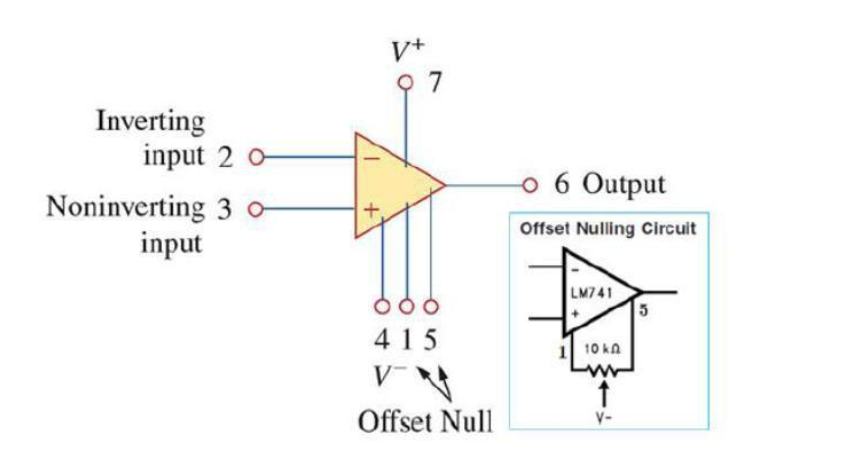
\includegraphics[width=0.7\linewidth]{pic1}
	\caption{Circuit symbol of a typical op amp.}
	\label{fig:pic1}
\end{figure}
In Fig 1, there are:

Two terminals for input signals: inverting (labeled -) and non-inverting (labeled +)

A terminal for the output signal.

Two terminals for the power supply voltages: positive +Vcc and negative –Vcc. (e.g.
In this lab, set +Vcc = 5V; -Vcc = -5V. )

Accordingly, for LM741 op amp chip you see in reality, the pin numbers are shown in
Fig2:
\begin{figure}[H]
	\centering
	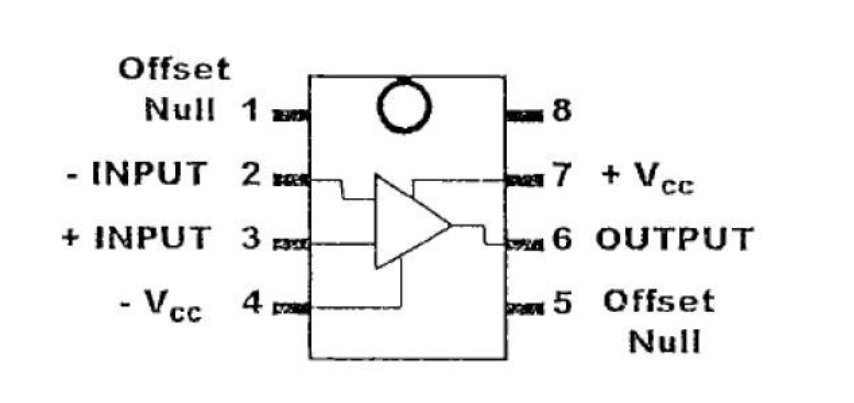
\includegraphics[width=0.7\linewidth]{pic2}
	\caption{Pin numbers for LM 741 op amp}
	\label{fig:pic2}
\end{figure}
\subsubsection{The gain of amplifier circuits}
The amplifier circuits are characterized by their gain values. The voltage gain is the
ratio of output voltage to the input voltage in the circuit:
$$VoltageGain=\frac{OutputVoltage}{InputVoltage}$$
In the lab, you can use oscilloscope to measure the input and output peak-to-peak (ppk)
amplitudes of the signals through two channels at the same time.
\subsubsection{Inverting amplifier}
\begin{figure}
	\centering
	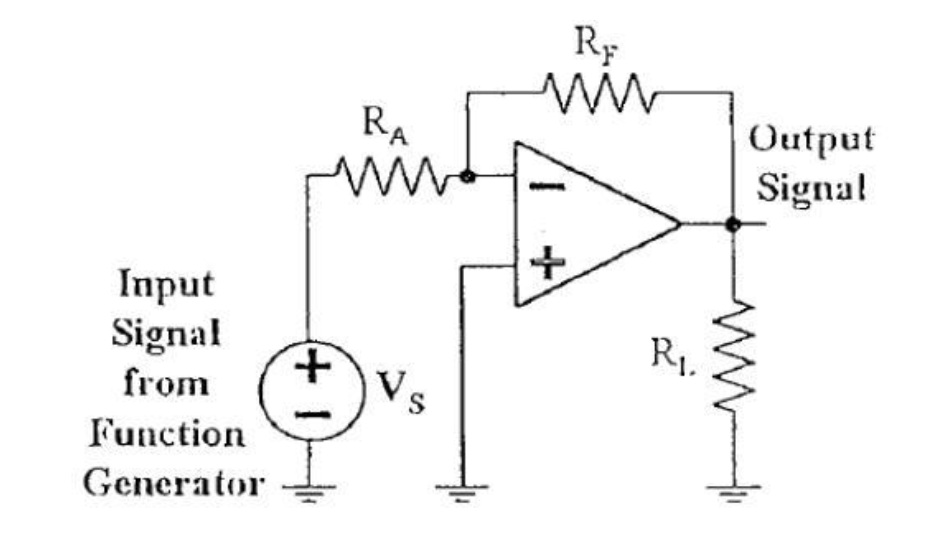
\includegraphics[width=0.7\linewidth]{pic3}
	\caption{ Inverting amplifier.}
	\label{fig:pic3}
\end{figure}
For inverting amplifier, the theoretical gain should be:
$$Gain=\frac{V_{output}}{V_s}=-\frac{R_F}{R_A}$$
\subsubsection{Non-inverting amplifier}
\begin{figure}[H]
	\centering
	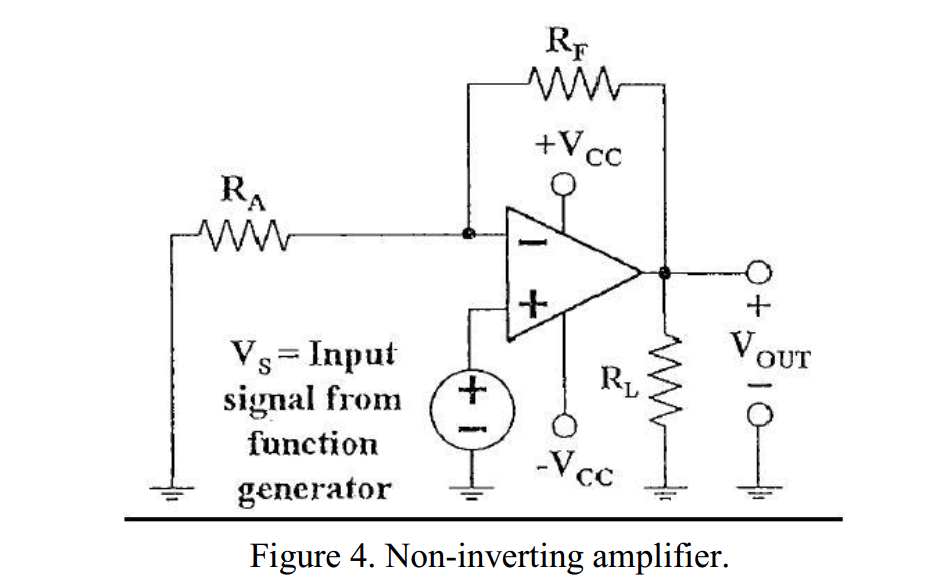
\includegraphics[width=0.7\linewidth]{pic4}
	\caption{Non-inverting amplifier.}
	\label{fig:pic4}
\end{figure}
For non-inverting amplifier, the theoretical gain should be:
$$Gain=\frac{V_{output}}{V_S}=1+\frac{R_F}{R_A}$$
\subsection{Appratus}
\subsubsection{Function generator}
Check the next page about the main buttons we would use
\begin{figure}[H]
	\centering
	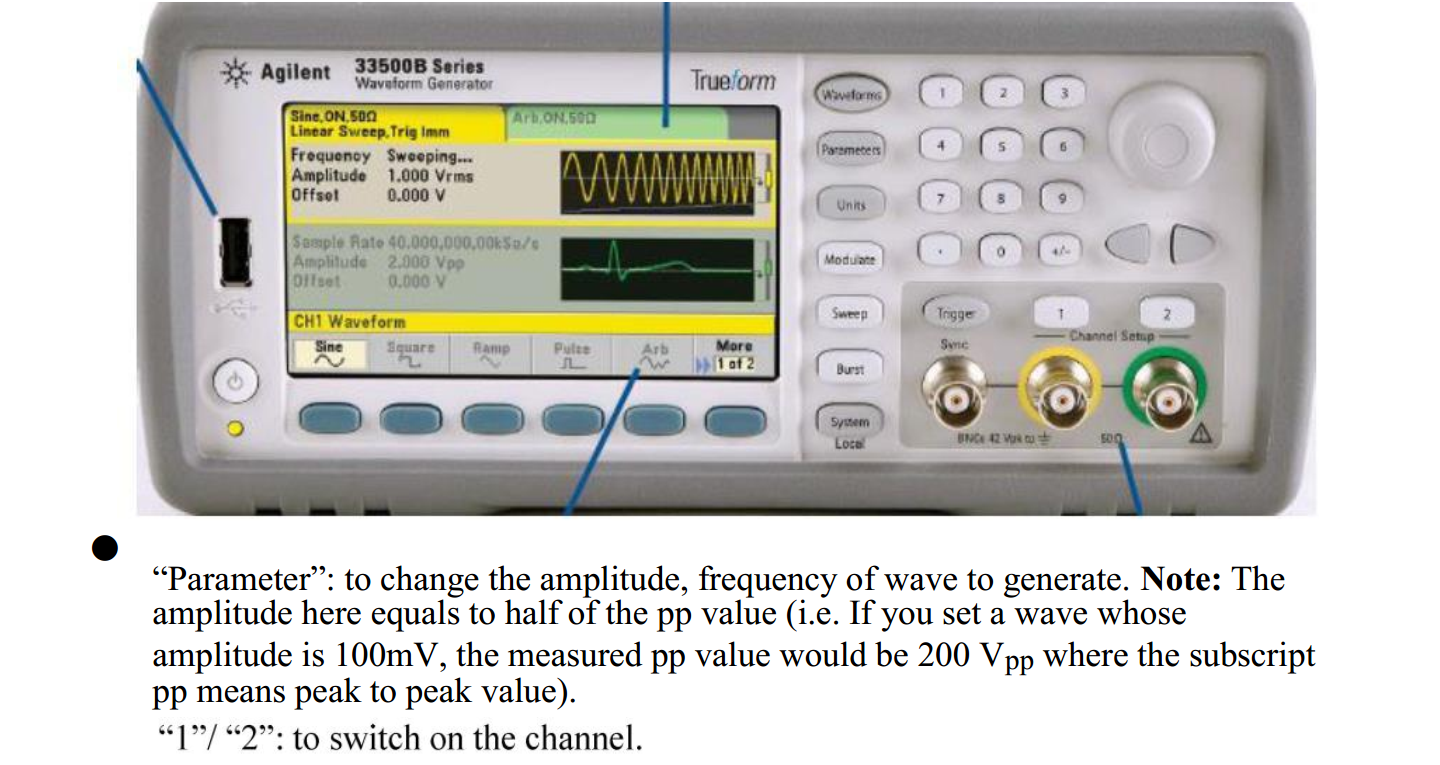
\includegraphics[width=0.7\linewidth]{pic5}
	\label{fig:pic5}
\end{figure}
\subsubsection{Oscilloscope}
\begin{figure}[H]
	\centering
	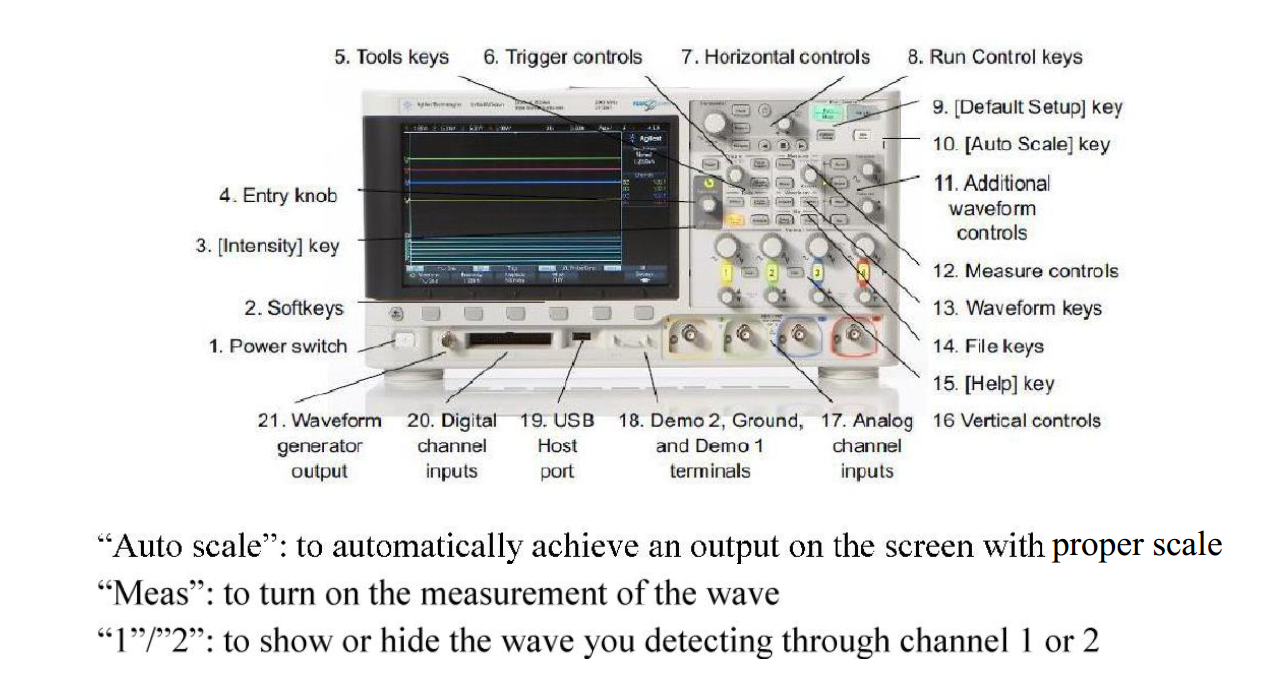
\includegraphics[width=0.7\linewidth]{pic6}
	\label{fig:pic6}
\end{figure}
\section{Non-inverting Amplifier}
\begin{table}[H]
	\centering
	\begin{tabular}{|c|c|}
		\hline
		$R_1[\Omega]$&50.9\\
		\hline
		$R_f[\Omega]$&99.6\\
		\hline
	\end{tabular}
	\caption{Resistances}
\end{table}
\begin{table}[H]
	\centering
	\begin{tabular}{|c|c|}
		\hline
		$+Vcc[V]$&5\\
		\hline
		$-Vcc[V]$&-5\\
		\hline
	\end{tabular}
	\caption{Voltage Supply to the Op Amp}
\end{table}
\begin{table}[H]
	\centering
	\begin{tabular}{|c|c|}
		\hline
		$V_{pp(in)}[V]$&$V_{pp(out)}[V]$\\
		\hline
		0.1&0.34\\
		\hline
		0.2&0.62\\
		\hline
		0.3&0.91\\
		\hline
		0.4&1.26\\
		\hline
		0.5&1.50\\
		\hline
		0.6&1.84\\
		\hline
		0.7&2.11\\
		\hline
		0.8&2.43\\
		\hline
		0.9&2.71\\
		\hline
		1.0&3.0\\
		\hline
		1.1&3.37\\
		\hline
		1.2&3.62\\
		\hline
		1.3&3.75\\
		\hline
		1.4&3.81\\
		\hline
		1.5&3.83\\
		\hline
	\end{tabular}
	\caption{The Input-Output Relationship}
\end{table}
\begin{figure}[H]
	\centering
	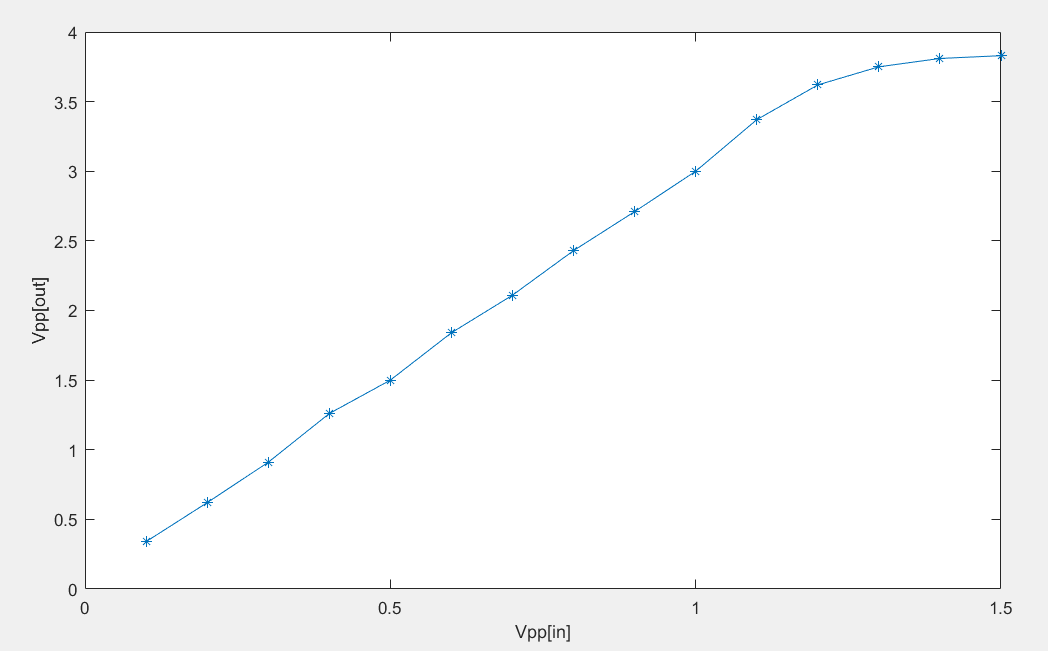
\includegraphics[width=0.7\linewidth]{noninverting}
	\caption{The relationship between Vout and Vin}
	\label{fig:noninverting}
\end{figure}
Just take the V from 0.1 to 0.9 we can get that 
\begin{figure}[H]
	\centering
	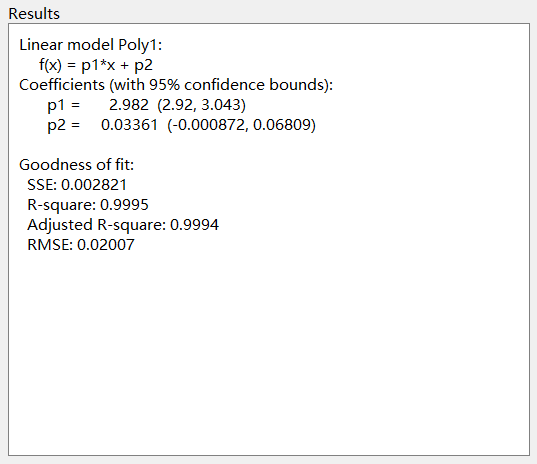
\includegraphics[width=0.7\linewidth]{noninvertingcf}
	\caption{the output of non-inverting amplifier}
	\label{fig:noninvertingcf}
\end{figure}
The figure below is about the relationship between the Gain and the Vin.
\begin{figure}[H]
	\centering
	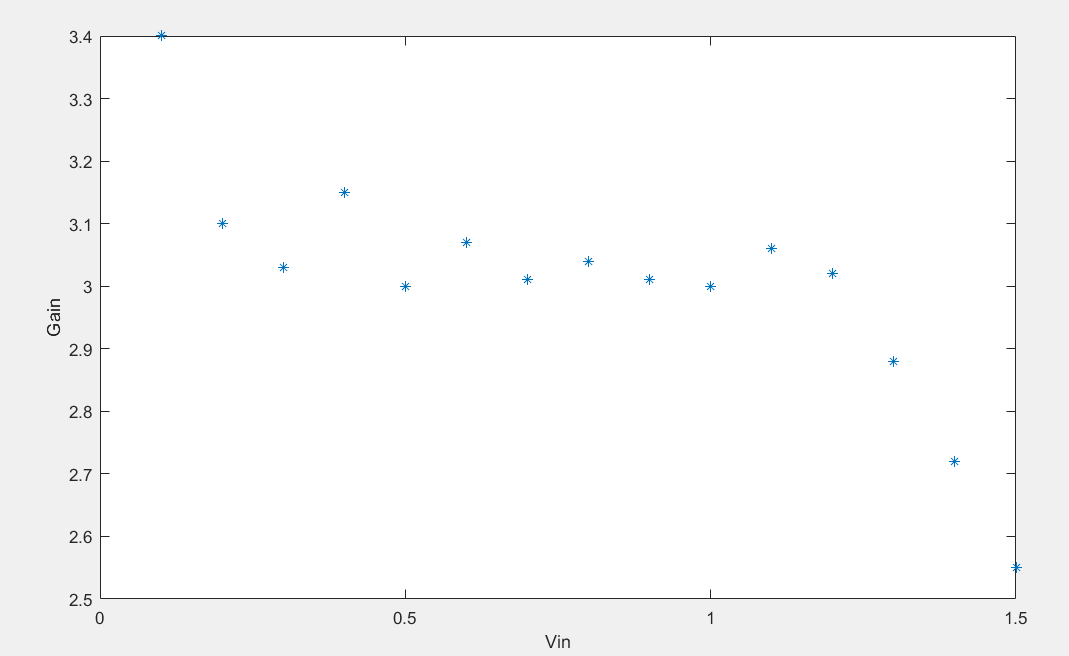
\includegraphics[width=0.7\linewidth]{gv1}
	\caption{The relationship between the gain and Vin}
	\label{fig:gv1}
\end{figure}

\section{Inverting Amplifier}
\begin{table}[H]
	\centering
	\begin{tabular}{|c|c|}
		\hline
		$R_1[\Omega]$&50.9\\
		\hline
		$R_f[\Omega]$&99.6\\
		\hline
	\end{tabular}
	\caption{Resistances}
\end{table}
\begin{table}[H]
	\centering
	\begin{tabular}{|c|c|}
		\hline
		$+Vcc[V]$&5\\
		\hline
		$-Vcc[V]$&-5\\
		\hline
	\end{tabular}
	\caption{Voltage Supply to the Op Amp}
\end{table}
\begin{table}[H]
	\centering
	\begin{tabular}{|c|c|}
		\hline
		$V_{pp(in)}[V]$&$V_{pp(out)}[V]$\\
		\hline
		0.1&0.221\\
		\hline
		0.2&0.418\\
		\hline
		0.3&0.615\\
		\hline
		0.4&0.830\\
		\hline
		0.5&1.02\\
		\hline
		0.6&1.22\\
		\hline
		0.7&1.42\\
		\hline
		0.8&1.61\\
		\hline
		0.9&1.80\\
		\hline
		1.0&2.05\\
		\hline
		1.1&2.25\\
		\hline
		1.2&2.47\\
		\hline
		1.3&2.65\\
		\hline
		1.4&2.85\\
		\hline
		1.5&3.06\\
		\hline
		1.6&3.26\\
		\hline
		1.7&3.440\\
		\hline
		1.8&3.660\\
		\hline
		1.9&3.840\\
		\hline
		2.0&4.020\\
		\hline
		2.1&4.30\\
		\hline
		2.2&4.460\\
		\hline
		2.3&4.60\\
		\hline
		2.4&4.820\\
		\hline
		2.5&4.94\\
		\hline
		2.6&5.07\\
		\hline
		2.7&5.15\\
		\hline
		2.8&5.31\\
		\hline
		2.9&5.39\\
		\hline
		3.0&5.43\\
		\hline
	\end{tabular}
	\caption{The Input-Output Relationship}
\end{table}
\begin{figure}[H]
	\centering
	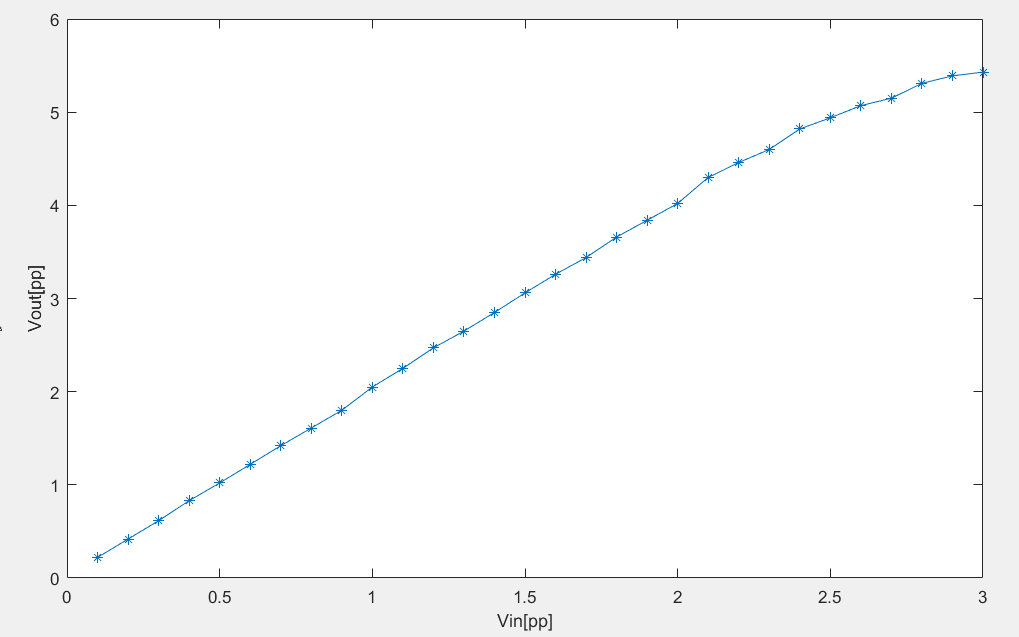
\includegraphics[width=0.7\linewidth]{inverting}
	\caption{The Input-Output Relationship}
	\label{fig:inverting}
\end{figure}
Just take the V from 0.1 to 0.9 we can get that 
\begin{figure}[H]
	\centering
	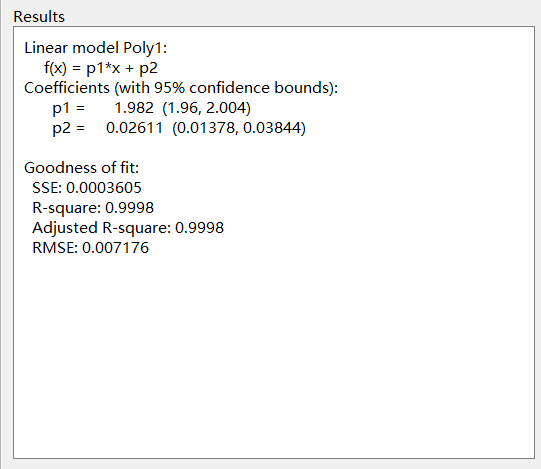
\includegraphics[width=0.7\linewidth]{invertingcf}
	\caption{the output of inverting amplifier	}
	\label{fig:invertingcf}
\end{figure}
The figure below is about the relationship between the Gain and the Vin.
\begin{figure}[H]
	\centering
	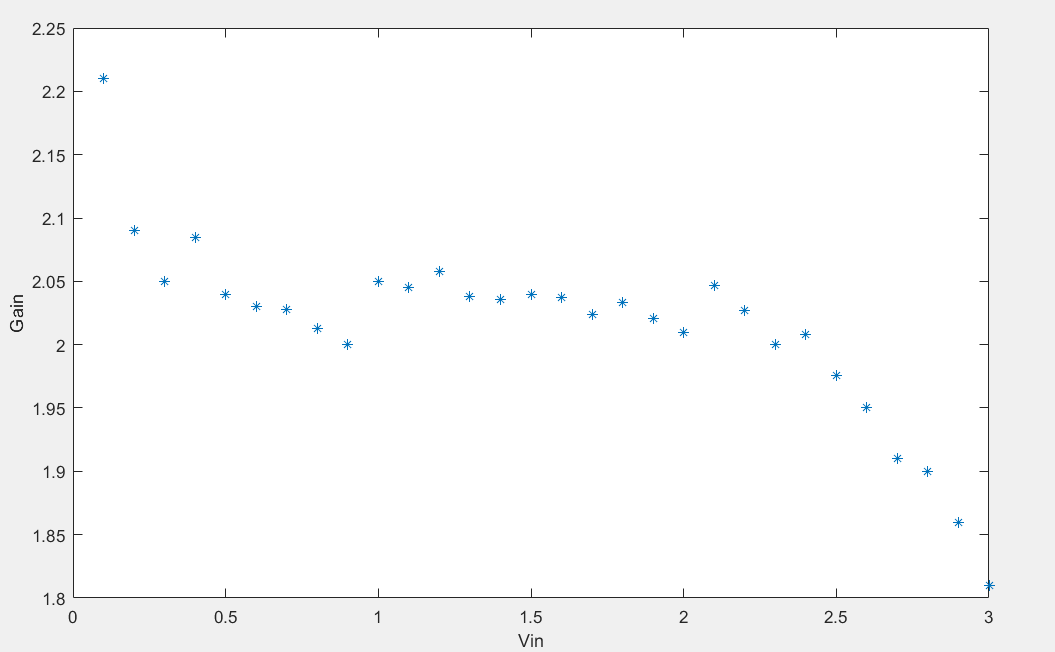
\includegraphics[width=0.7\linewidth]{gv2}
	\caption{The relationship between Gain and Vin}
	\label{fig:gv2}
\end{figure}
\section{Result}
From this experiment, we have learned to build and test a variety of circuits based on LM741 Op Amp chip: non-inverting and inverting amplifiers with fixed gain.  We also measure the gain of the amplifier and compare it with theoretical calculations.
\begin{enumerate}
\item From this part of the experiment, we can know that the result is relatively correct. When comparing the data from $Vin=0.1V$ to $Vin=0.9V$, we can know that the average of gain is $3.09$. Compared with the expected data, we can know that th error is about $3\%$. And actually it is not very big. Actually, this kind of result doesn't have a very big error. The reason why I don't take the value when $Vin>0.9V$ is that the outcome is about the saturated voltage. In this experiment, because that there are some errors about the equipments we are using, therefore, it seems to be very difficult to measure the absolutely correct saturated output voltage. And in our experiment, it is about $Vout=3.83V$ when $Vin=1.5V$. It is not absolutely correct because that when we were doing the experiment, we find that the what the equipment shows about the $Vout$ is about 13times of the expected value. And it is always shifting in two numbers when $Vin=1.5V$. Therefore, it seems that we can't get a very nice data and result in this experiment.

\item From this part of the experiment, we can know that the result is relatively correct. When comparing the data from $Vin=0.1V$ to $Vin=0.9V$, we can know that the average of gain is $2.06$. Compared with the expected data, we can know that th error is about $3\%$. And actually it is not very big. Actually, this kind of result doesn't have a very big error.  The reason why I don't take the value when $Vin>0.9V$ is that the outcome is about the saturated voltage. In this part, out team changes to another desk to test the second part and I think the equipments are much more accurate. In our experiment, we found that when the $Vin=2.9V$ and $Vin=2.0V$, the rise of the $Vout$ is nt very big. And because of the limitation of time, we don't have more time to test more data. But this is enough to illustrate that this is the saturated voltage.
\end{enumerate}


This experiment is a little bit tough to do because that some of the equipments are not absolutely correct. However, I think that the outcome is still relatively correct. I think the lab should use some good equipments instead of some equipments that have problems. And during the lab, TA provides two kinds of Op Amp. And it seems that we use another one and use the LM741 method to connect the circuit at the first time. Therefore, it seems that I still need to be more careful when doing the experiment.


In general, the experiment is very meaningful. It makes us have a better understanding about the inverting and non-inverting amplifiers. And we know more about its gain. But we still have some difficulties when doing the lab.
\begin{figure}[H]
	\centering
	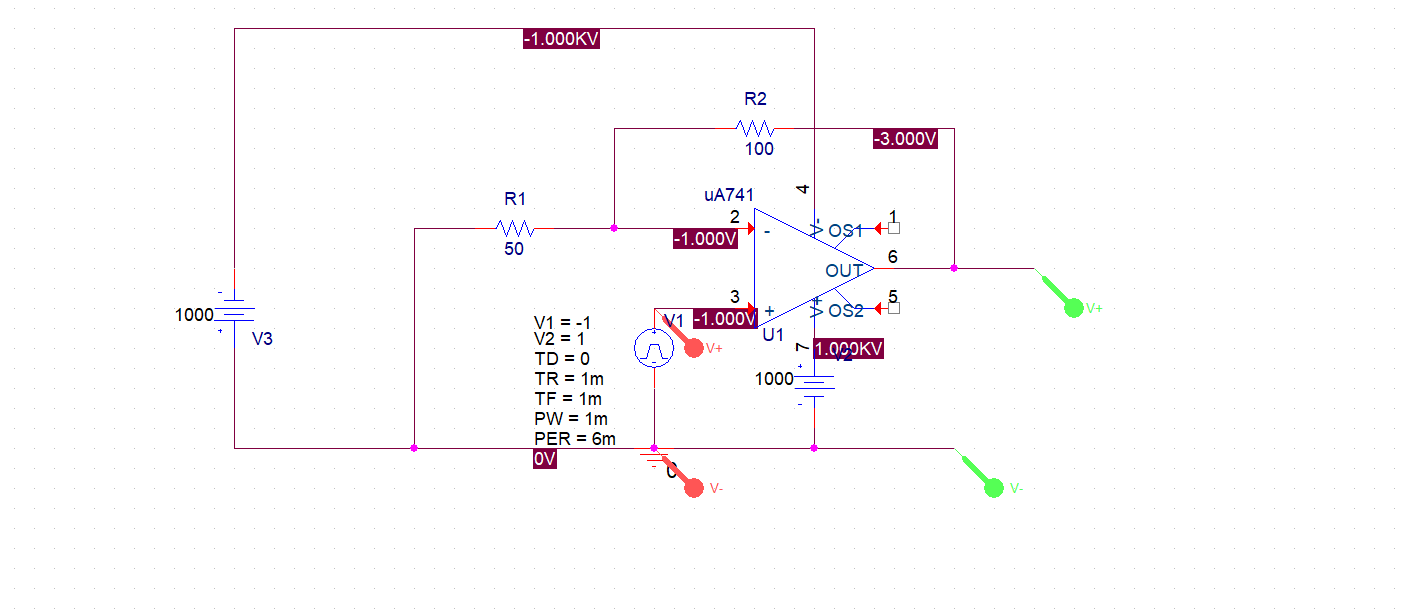
\includegraphics[width=0.7\linewidth]{bonus11}
	\caption{Non-inverting Amplifier 1}
	\label{fig:bonus11}
\end{figure}
\begin{figure}[H]
	\centering
	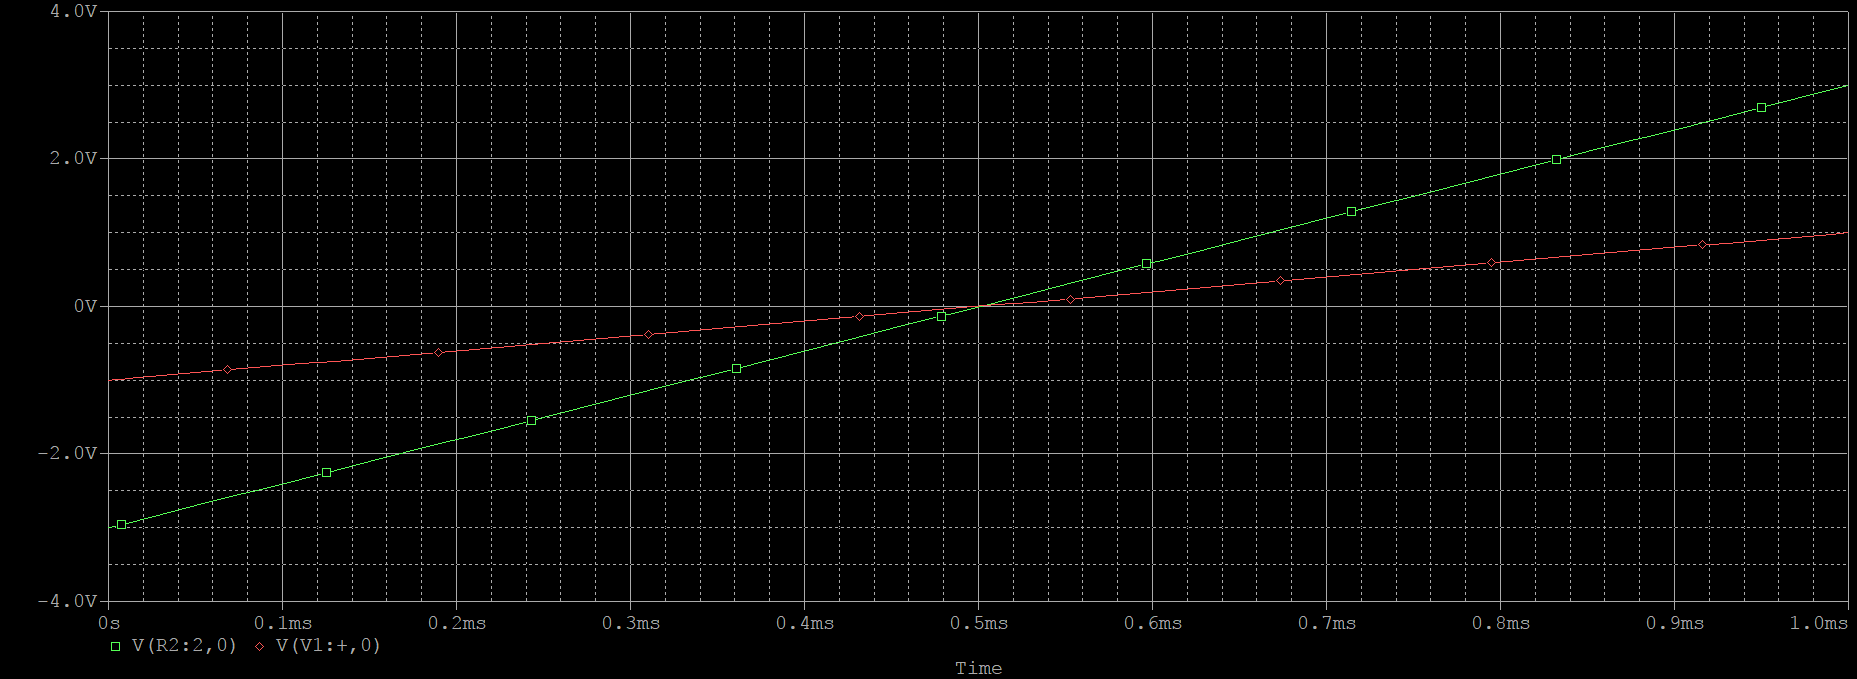
\includegraphics[width=0.7\linewidth]{bonus12}
	\caption{Non-inverting Amplifier 2}
	\label{fig:bonus12}
\end{figure}
\begin{figure}[H]
	\centering
	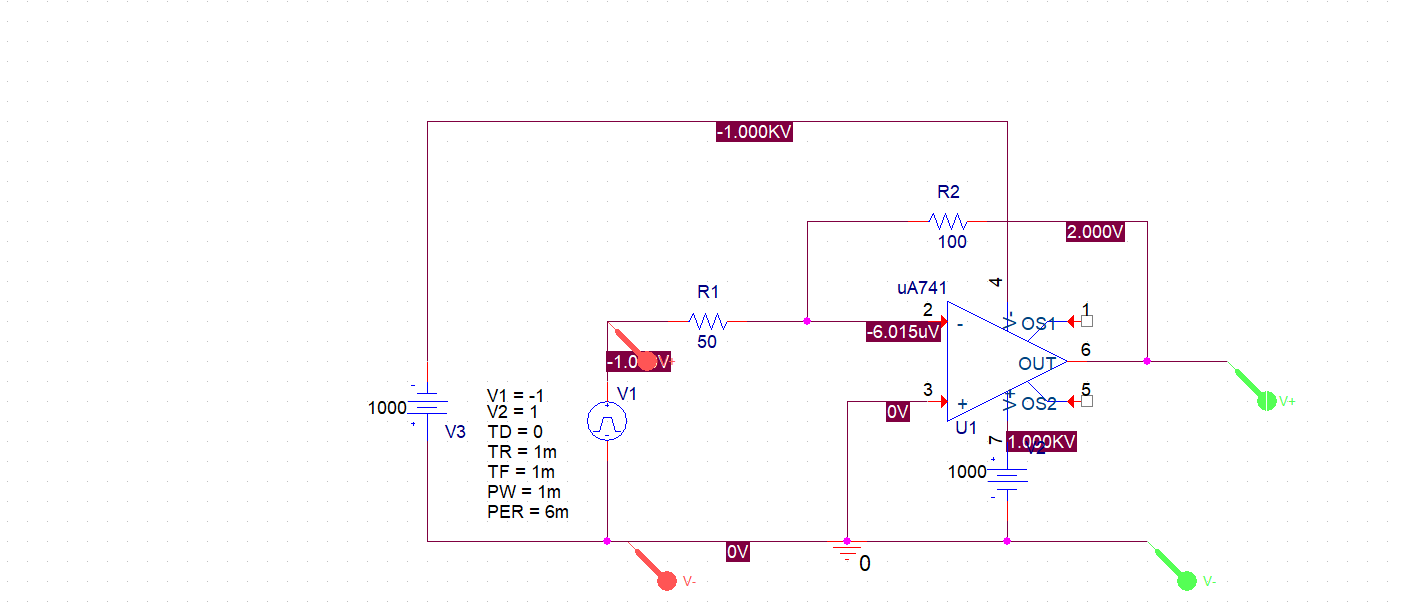
\includegraphics[width=0.7\linewidth]{bonus21}
	\caption{Inverting Amplifier 1}
	\label{fig:bonus21}
\end{figure}
\begin{figure}[H]
	\centering
	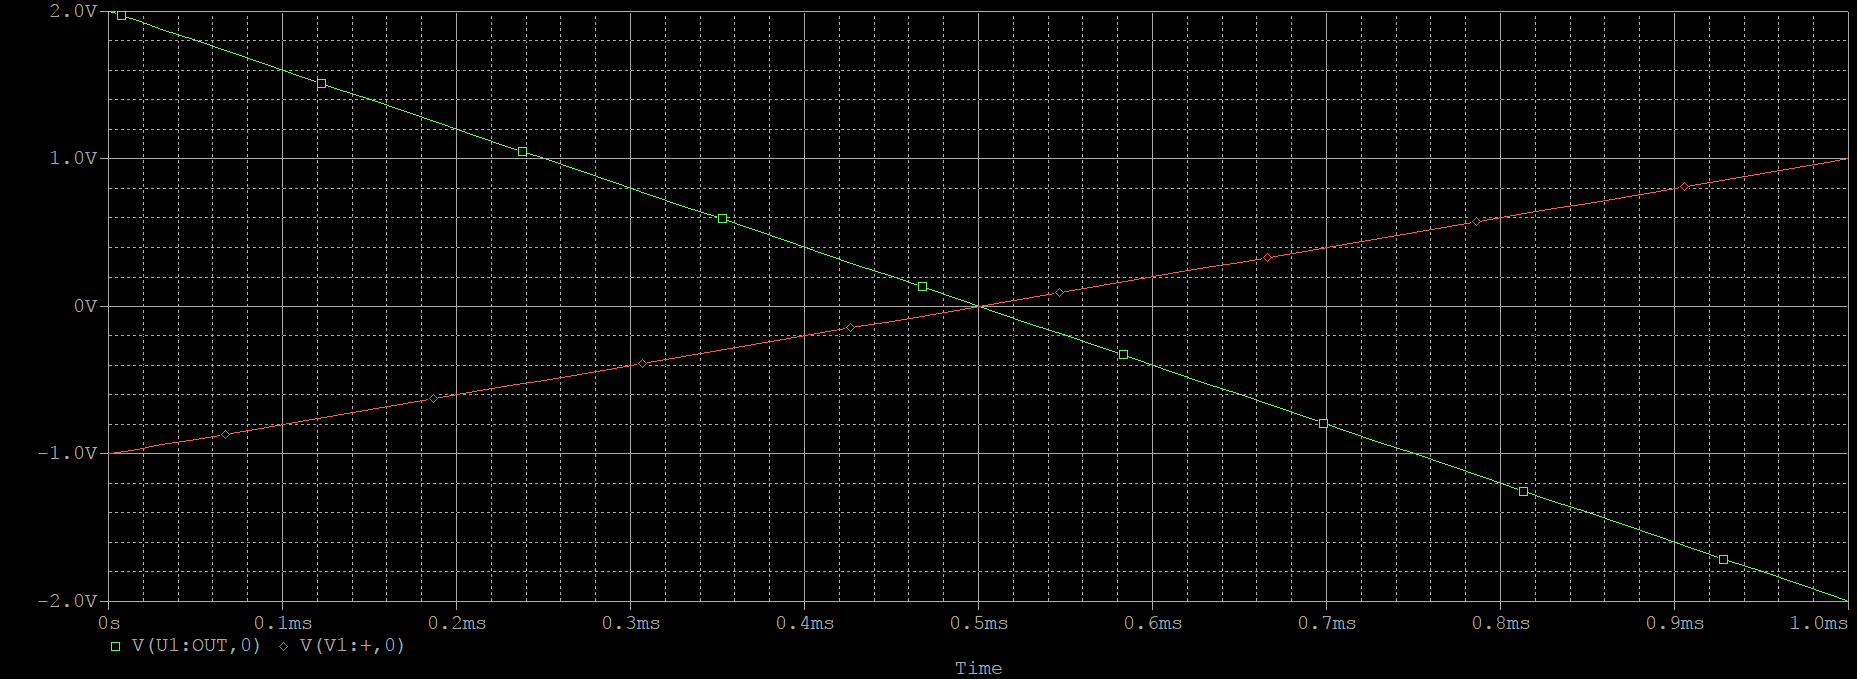
\includegraphics[width=0.7\linewidth]{bonus22}
	\caption{Inverting Amplifier 2}
	\label{fig:bonus22}
\end{figure}

\end{document}